%%%%%%%%%%%%%%%%%%%%%%%%%%%%%%%%%%%%%%%%%
% AYAB-Shield
% Soldering Manual - German
% Version 0.1 (17.11.2015)
%
% http://www.ayab-knitting.com
%
% Original author:
% Andreas Mueller (andreas.mueller@thinkstack.de)
%
% License:
% CC BY-SA 4.0 (http://creativecommons.org/licenses/by-sa/4.0/)
%
% LaTeX Template
%
% This template has been downloaded from:
% http://www.LaTeXTemplates.com
%
% Original author:
% Mathias Legrand (legrand.mathias@gmail.com)
%
% License:
% CC BY-NC-SA 3.0 (http://creativecommons.org/licenses/by-nc-sa/3.0/)
%
%%%%%%%%%%%%%%%%%%%%%%%%%%%%%%%%%%%%%%%%%

%----------------------------------------------------------------------------------------
%	PACKAGES AND OTHER DOCUMENT CONFIGURATIONS
%----------------------------------------------------------------------------------------

\documentclass[fleqn,10pt]{SelfArx} % Document font size and equations flushed left
%\documentclass{article}
%\usepackage{lipsum} % Required to insert dummy text. To be removed otherwise

%----------------------------------------------------------------------------------------
%	COLUMNS
%----------------------------------------------------------------------------------------

\setlength{\columnsep}{0.55cm} % Distance between the two columns of text
\setlength{\fboxrule}{0.75pt} % Width of the border around the abstract

%----------------------------------------------------------------------------------------
%	COLORS
%----------------------------------------------------------------------------------------

\definecolor{color1}{RGB}{0,0,90} % Color of the article title and sections
\definecolor{color2}{RGB}{0,20,20} % Color of the boxes behind the abstract and headings

%----------------------------------------------------------------------------------------
%	Packages
%----------------------------------------------------------------------------------------
\usepackage{textgreek} % Required for Omega
\usepackage{placeins} % Requierd for FloatBarrier
\usepackage{wasysym} % für die benutzten Symbole
\usepackage{hyperref} % Required for hyperlinks
\hypersetup{hidelinks,colorlinks,breaklinks=true,urlcolor=color2,citecolor=color1,linkcolor=color1,bookmarksopen=false,pdftitle={Title},pdfauthor={Author}}

\graphicspath{ {./images/} }
%----------------------------------------------------------------------------------------
%	ARTICLE INFORMATION
%----------------------------------------------------------------------------------------

\JournalInfo{AYAB-Shield Lötanleitung, v0.1, 2015-11-15} % Journal information
\Archive{CC BY-SA 4.0} % Additional notes (e.g. copyright, DOI, review/research article)

\PaperTitle{AYAB-Shield Lötanleitung} % Article title

\Authors{ayab-knitting.com} % Authors
%\affiliation{\textsuperscript{1}\textit{Department of Biology, University of Examples, London, United Kingdom}} % Author affiliation
%\affiliation{\textsuperscript{2}\textit{Department of Chemistry, University of Examples, London, United Kingdom}} % Author affiliation
%\affiliation{*\textbf{Corresponding author}: john@smith.com} % Corresponding author

\Keywords{} % Keywords - if you don't want any simply remove all the text between the curly brackets
\newcommand{\keywordname}{Keywords} % Defines the keywords heading name

%----------------------------------------------------------------------------------------
%	ABSTRACT
%----------------------------------------------------------------------------------------

\Abstract{

Bei Schäden, die durch Nichtbeachtung der Bedienungsanleitung entstehen, erlischt jeglicher Gewährleistungsanspruch. Für Folgeschäden, die daraus resultieren, übernehmen wir keine Haftung

}

%----------------------------------------------------------------------------------------

\begin{document}

\flushbottom % Makes all text pages the same height

\maketitle % Print the title and abstract box

\tableofcontents % Print the contents section

\thispagestyle{empty} % Removes page numbering from the first page

%----------------------------------------------------------------------------------------
%	ARTICLE CONTENTS
%----------------------------------------------------------------------------------------

\section*{Hinweis} % The \section*{} command stops section numbering

%\addcontentsline{toc}{section}{Introduction} % Adds this section to the table of contents

Derjenige, der einen Bausatz fertigstellt oder eine Baugruppe durch Erweiterung bzw. Gehäuseeinbau betriebsbereit macht, gilt nach DIN VDE 0869 als Hersteller und ist verpflichtet, bei der Weitergabe des Gerätes alle Begleitpapiere mitzuliefern und auch seinen Namen und Anschrift anzugeben. Geräte, die aus Bausätzen selbst zusammengestellt werden, sind sicherheitstechnisch wie ein industrielles Produkt zu betrachten.

%------------------------------------------------

\section{Betriebsbedingungen}

\begin{itemize}[noitemsep] % [noitemsep] removes whitespace between the items for a compact look
\item Dieser Bausatz ist nicht für den Einsatz in Lebenserhaltenden oder lebensrettenden Systemen oder ähnlichen Anwendungen konzipiert! Verwenden Sie das Produkt nicht für Zwecke, bei denen im Falle eines Ausfalls, einer Störung oder einer Fehlfunktion Personen- oder Sachschaden möglich sind.
\item Wird der Baustein zum Schalten hoher Spannungen (mehr als 24V) verwendet, darf die Elektroinstallation nur in spannungslosem Zustand
und nur durch einen sachkundigen Fachmann erfolgen. Der Baustein/Bausatz darf nur dann in Betrieb genommen werden, wenn er vorher berührungssicher in ein Gehause eingebaut wurde.
\item Der Baustein ist ausschließlich für den Einsatz in trockener und sauberer Umgebung geeignet. Die Verwendung in unmittelbarer Umgebung leicht brennbaren Gegenständen, von Wasser, grobem Schmutz oder starker Feuchtigkeit ist gefährlich und unzulässig.
\item Das Produkt darf nicht in Verbindung oder in der Nähe mit leicht entflammbaren und brennbaren Flüssigkeiten verwendet werden.
\item überschreiten Sie keinesfalls die elektrischen Grenzwerte, die unter “Technische Daten“ am Ende dieser Anleitung angegeben sind.
\item In Schulen, Ausbildungseinrichtungen, Hobby- und Selbsthilfewerkstätten ist das Betreiben von Modulen und Bausteinen von geschultem Personal verantwortlich zu Überwachen.
\item Das Produkt ist kein Spielzeug und kann für Kinder gefährlich sein! (Verschlucken von Kleinteilen, Stromschlag usw.)
\item Baugruppen und Bauteile gehören nicht in Kinderhände!
\item Die Baugruppen dürfen nur unter Aufsicht eines fachkundigen Erwachsenen oder eines Fachmannes in Betrieb genommen werden!
\item In gewerblichen Einrichtungen sind die Vorschriften zur Unfallverhütung des Verbandes der gewerblichen Berufsgenossenschaften für elektrische Anlagen und Betriebsmittel zu beachten.
\item Eine Reparatur des Gerätes darf nur vom Fachmann durchgeführt werden!
\item Dringt irgendeine Flüssigkeit in das Gerät ein, so könnte es dadurch beschädigt werden. Sollten Sie irgendwelche Flüssigkeiten in, oder über die Baugruppe verschüttet haben, so muss das Gerät von einem qualifizierten Fachmann überprüft werden

\end{itemize}

%------------------------------------------------

\section{Bestimmungsgemäße Verwendung}

Der bestimmungsgemäße Einsatz des fertiggestellten Bausatzes ist die Steuerung von Brother Heimstrickmaschinen der KH-9xx Serie. Es darf nur als Ersatz der vorhandenen Steuerplatine eingesetzt werden. Ein parallelbetrieb mit der Originalsteuerung ist nicht vorgesehen.

Ein anderer Einsatz als vorgegeben ist nicht zulässig!

%------------------------------------------------

\section{Sicherheitshinweise}

Beim Umgang mit Produkten, die mit elektrischer Spannung in Berührung kommen, müssen die gültigen VDE-Vorschriften beachtet werden, insbesondere VDE 0100, VDE 0550/0551, VDE 0700, VDE 0711 und VDE 0860.
\begin{itemize}[noitemsep] % [noitemsep] removes whitespace between the items for a compact look
\item Vor Öffnen eines Gerätes stets den Netzstecker ziehen oder sicherstellen, daß das Gerät stromlos ist.
\item Bauteile, Baugruppen oder Geräte dürfen nur in Betrieb genommen werden, wenn sie vorher berührungssicher in ein Gehäuse eingebaut wurden. Während des Einbaus müssen sie stromlos sein.
\item Werkzeuge dürfen an Geräten, Bauteilen oder Baugruppen nur benutzt werden, wenn sichergestellt ist, dass die Geräte von der Versorgungsspannung getrennt sind und elektrische Ladungen, die in den im Gerät befindlichen Bauteilen gespeichert sind, vorher entladen wurden.
\item Spannungsführende Kabel oder Leitungen, mit denen das Gerät, das Bauteil oder die Baugruppe verbunden ist, müssen stets auf Isolationsfehler oder Bruchstellen untersucht werden. Bei Feststellen eines Fehlers in der Zuleitung muss das Gerät unverzüglich aus dem Betrieb genommen werden, bis die defekte Leitung ausgewechselt worden ist.
\item Bei Einsatz von Bauelementen oder Baugruppen muss stets auf die strikte Einhaltung der in der zugehörigen Beschreibung genannten Daten für elektrische Größen hingewiesen werden.
\item Wenn aus einer vorliegenden Beschreibung für den nichtgewerblichen Endverbraucher nicht eindeutig hervorgeht, welche elektrischen Kennwerte für ein Bauteil oder eine Baugruppe gelten, wie eine externe Beschaltung durchzuführen ist oder welche externen Bauteile oder Zusatzgeräte angeschlossen werden dürfen und welche Anschlußwerte diese externen Komponenten haben dürfen, so muss stets ein Fachmann um Auskunft ersucht werden.
\item Es ist vor der Inbetriebnahme eines Gerätes generell zu prüfen, ob dieses Gerät oder Baugruppe grundsätzlich für den Anwendungsfall, für den es verwendet werden soll, geeignet ist! Im Zweifelsfalle sind unbedingt Rückfragen bei Fachleuten, Sachverständigen oder den Herstellern der verwendeten Baugruppen notwendig!
\item Bitte beachten Sie, dass Bedien- und Anschlussfehler außerhalb unseres Einflussbereiches liegen. \par Verständlicherweise können wir für Schäden, die daraus entstehen, keinerlei Haftung übernehmen.
\item Bausätze sollten bei Nichtfunktion mit einer genauen Fehlerbeschreibung und der zugehörigen Bauanleitung sowie ohne Gehäuse zurückgesandt werden. Zeitaufwendige Montagen oder Demontagen von Gehäusen müssen wir aus verständlichen Gründen zusätzlich berechnen. Bereits aufgebaute Bausätze sind vom Umtausch ausgeschlossen. Bei Installationen und beim Umgang mit Netzspannung sind unbedingt die VDE-Vorschriften zu beachten.
\item Geräte, die an einer Spannung über 24 V betrieben werden, dürfen nur vom Fachmann angeschlossen werden.
\item Die Inbetriebnahme darf grundsätzlich nur erfolgen, wenn die Schaltung absolut berührungssicher in ein Gehäuse eingebaut ist.
\item Sind Messungen bei geöffnetem Gehäuse unumgänglich, so muss aus Sicherheitsgründen ein Trenntrafo zwischengeschaltet werden, oder, wie bereits erwähnt, die Spannung über ein geeignetes Netzteil, (das den Sicherheitsbestimmungen entspricht) zugeführt werden.
\item Alle Verdrahtungsarbeiten dürfen nur im spannungslosen Zustand ausgeführt werden.

\end{itemize}

%------------------------------------------------

\section{Produktbeschreibung}

AYAB – all yarns are beautiful ermöglicht es, die bekannten Strickmaschinenmodelle Brother KH-910 und KH-930 (und kompatible) über einen USB Anschluss mit dem Computer zu verbinden. Dadurch eröffnen sich völlig neue Möglichkeiten für die Geräte, denn damit können selbst erstellte Bilddateien direkt an der Maschine ausgestrickt werden. Ein Einlesen von Bildkarten (KH-910/950), oder das manuelle Einprogrammieren von Mustern (KH-930 und andere) entfällt damit.

Zudem werden die Fähigkeiten der Maschine erweitert, denn mit AYAB können Muster über die volle Breite der Maschine (200 Nadeln), anstatt wie bisher nur 60 Nadeln gestrickt werden.
Vor allem für das relativ kostengünstige Modell KH-910, das aufgrund seiner unzuverlässigen Scannereinheit ein Nischendasein fristet, kommt damit wieder zu neuer Funktion, die den moderneren Modellen mindestens gleichauf ist.

Für das AYAB Shield benötigt man einen handelsüblichen Arduino UNO oder MEGA (nicht im Lieferumfang enthalten). Für die Installation muss das Gehäuse des Gerätes geöffnet werden und lediglich einige der vorhandenen Kabel von der bisherigen Steuereinheit auf das AYAB Shield umgesteckt werden (siehe Anleitungsvideo).

Die Installation von AYAB ist voll reversibel. Werden die Kabel wieder auf die originale Steuereinheit zurückgesteckt, funktioniert die Strickmaschine wieder wie im Originalzustand.

Der Arduino muss zur Inbetriebnahme mit der aktuellen Version der AYAB Firmware bespielt werden. Diese ist [hier] (Modell beachten!) bereits vorkompiliert verfügbar und muss nur noch auf den Arduino übertragen werden (siehe Anleitungsvideo).

Das AYAB Projekt ist freie und offene Soft- und Hardware. Der komplette Quellcode und die Layoutdateien sind frei verfügbar und zur Anpassung an eigene Bedürfnisse freigegeben. Natürlich freut sich das AYAB Team über jegliches Feedback und Mitarbeit am Projekt.

 \subsection*{Eigenschaften}

Unterstützte Modelle: Brother KH-910, Brother KH-930 (weitere Modelle werden demnächst offiziell hinzugefügt)
Maximale Musterbreite: 200 Nadeln
Maximale Musterlänge: unbegrenzt
Maximale Anzahl der Farben: 2 (bis zu 6 experimentell)

 \subsection*{Hinweis}

Bitte bei der Bestellung auf den richtigen Maschinentyp achten. Nur so kann gewährleistet werden, dass kompatible Steckverbindungen mitgeliefert werden.

%------------------------------------------------

\section{Technische Daten}

\begin{tabular}{ll}
Versorgungsspannung       & 5.0 V              \\ \hline
Schaltspannung            & 7.5V - 16.0V       \\ \hline
max. Stromaufnahme        & xxx mA             \\ \hline
max. Schaltstrom          & xxx mA             \\ \hline
Abmessungen (l x b x h)   & xxmm x yymm x zzmm
\end{tabular}


%------------------------------------------------

\section{Bevor Sie beginnen}

Bevor Sie mit dem Aufbau beginnen, lesen Sie diese Bauanleitung erst einmal bis zum Ende in Ruhe durch, bevor Sie den Bausatz oder das Gerät in Betrieb nehmen (besonders den Abschnitt über die Fehlermöglichkeiten und deren Beseitigung!) und natürlich die Sicherheitshinweise. Sie wissen dann, worauf es ankommt und was Sie beachten müssen und vermeiden dadurch von vornherein Fehler, die manchmal nur mit viel Aufwand wieder zu beheben sind!

Führen Sie die Lötungen und Verdrahtungen absolut sauber und gewissenhaft aus, verwenden Sie kein säurehaltiges Lötzinn, Lötfett o. ä. Vergewissern Sie sich, dass keine kalte Lötstelle vorhanden ist. Denn eine unsaubere Lötung oder schlechte Lötstelle, ein Wackelkontakt oder schlechter Aufbau bedeuten eine aufwendige und zeitraubende Fehlersuche und unter Umständen eine Zerstörung von Bauelementen, was oft eine Kettenreaktion nach sich zieht und der komplette Bausatz zerstört wird.

Beachten Sie auch, dass Bausätze, die mit säurehaltigem Lötzinn, Lötfett o. ä. gelötet wurden, von uns nicht repariert werden.

Beim Nachbau elektronischer Schaltungen werden Grundkenntnisse über die Behandlung der Bauteile, Löten und der Umgang mit elektronischen bzw. elektrischen Bauteilen vorausgesetzt.

 \subsection*{Allgemeine Hinweise}

Die Möglichkeit, dass nach dem Zusammenbau etwas nicht funktioniert, lässt sich durch einen gewissenhaften und sauberen Aufbau drastisch verringern. Kontrollieren Sie jeden Schritt, jede Lötstelle zweimal, bevor Sie weitergehen! Halten Sie sich an die Bauanleitung! Machen Sie den dort beschriebenen Schritt nicht Bei 90 \% der funktionsuntüchtigen Bausätze handelt es sich um Lötfehler, kalte Lötstellen, falsches Lötzinn usw. Verwenden Sie deshalb beim Löten nur Elektroniklötzinn mit der Bezeichnung “SN 60 Pb” (60 \% Zinn und 40 \% Blei). Dieses Lötzinn hat eine Kolophoniumseele, welche als Flussmittel dient, um die Lötstelle während des Lötens vor dem Oxydieren zu schützen. Andere Flussmittel wie Lötfett, Lötpaste oder Lötwasser dürfen auf keinen Fall verwendet werden, da sie säurehaltig sind. Diese Mittel können die Leiterplatte und Elektronik-Bauteile zerstören, außerdem leiten sie den Strom und verursachen dadurch Kriechströme und Kurzschlüsse.

Dieser Bausatz wurde, bevor er in Produktion ging, viele Male als Prototyp aufgebaut und getestet. Erst wenn eine optimale Qualität hinsichtlich Funktion und Betriebssicherheit erreicht ist, wird er für die Serie freigegeben.

%------------------------------------------------

\section{Montage der Bauelemente auf der Platine}

 \subsection*{Hinweis}

Beim Aufbau halten Sie sich an die Montageanleitung und werfen nebenbei immer einen Blick auf den Bestückungsplan.

Besonderes Augenmerk gilt den drei Leuchtdioden, bei denen unbedingt auf richtige Polarität zu achten ist.

Beachten Sie die Markierungskerbe der IC-Gehäuse Fassung. Diese muss mit dem Bestückungsplan übereinstimmen.

Kontrollieren Sie vor Inbetriebnahme der Schaltung die Position aller Bauteile.

Achten Sie beim Einlöten der Bauelemente darauf, daß diese (falls nicht Gegenteiliges vermerkt) ohne Abstand zur Platine eingelötet werden. Alle überstehenden Anschlussdrähte werden direkt über der Lötstelle abgeschnitten.

Da es sich bei diesem Bausatz teilweise um sehr kleine bzw. eng beieinanderliegende Lötpunkte handelt (Gefahr von Lötbrücken), darf hier nur mit einem Lötkolben mit kleiner Lötspitze gelötet werden. Führen Sie die Lötvorgänge und den Aufbau sorgfältig aus.

 \subsection*{Lötanleitung}

Wenn sie mit dem Löten noch nicht so vertraut sind, lesen Sie bitte eine geeignete Lötanleitung für bedrahtete Bauteile durch. Diese können Sie im Internet z.B. unter \url{http:\\example.com} finden.

Achten Sie darauf des es sich bei einigen Bauteilen (insbesondere die ICs) um temperaturempfindliche Bauteile handelt. Achten Sie deshalb auf eine möglichst kurze Aufheizzeit oder verwenden Sie eine IC-Fassung.

 \subsection*{Schritt 1: LEDs}


\begin{tabular}{ll}
\hline
\textbf{Name} & \textbf{Farbe} \\ \hline
LED1          & rot            \\ \hline
LED2          & gelb           \\ \hline
LED2          & grün           \\ \hline
\end{tabular}\\

Platzieren die drei LEDs (rot, gelb, grün) ensprechend der Abbildung \ref{fig:abb1_1} auf der Platine. Achten Sie dabei unbedingt auf die Richtige Polarität. Die Abgeflachte Gehäusekante der LED, bzw das kürzere Beinchen, müssen dabei weg von den Widerständen bzw. hin zum Platinenrand zeigen. Zusätzlich den Platinendruck beachten.

Im Anschluss werden diese von der Unterseite Verlötet.

\begin{figure}[tbhp]\centering
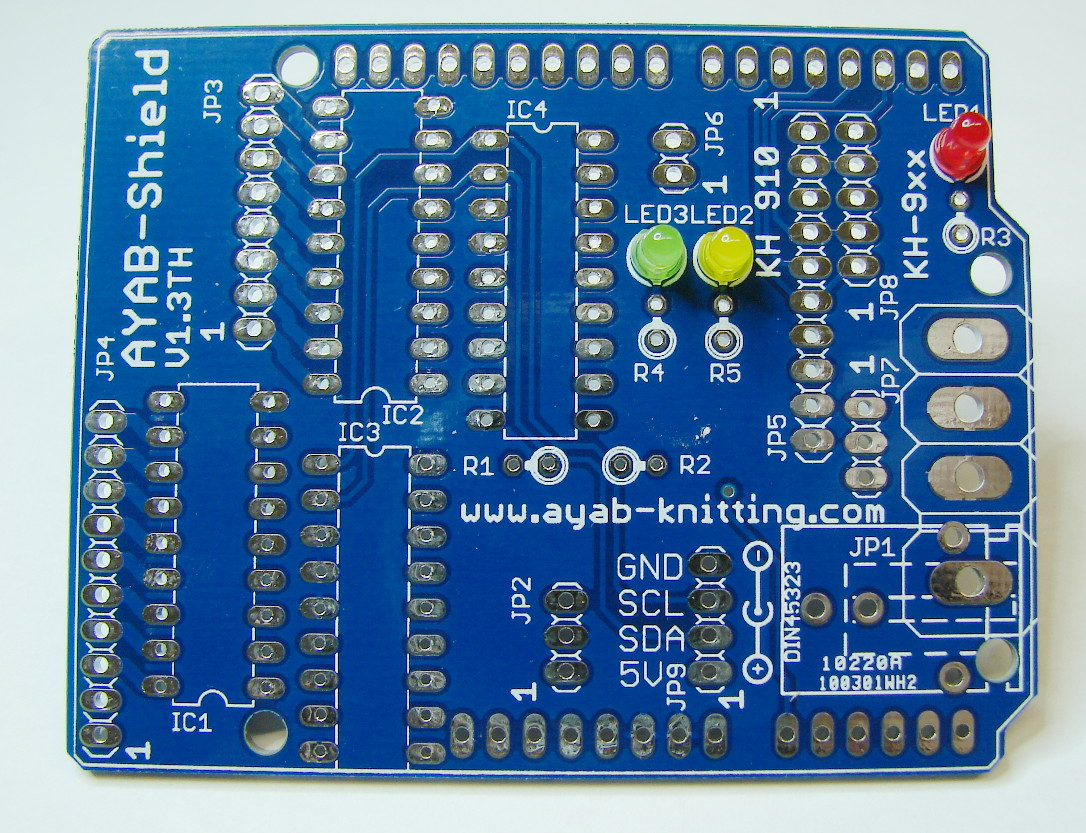
\includegraphics[width=\linewidth]{abb1_1}
\caption{LEDs}
\label{fig:abb1_1}
\end{figure}

\FloatBarrier

 \subsection*{Schritt 2: Widerstände}

Der AYAB-Shield Bausatz enthält zwei Widerstandstypen\\

\begin{tabular}{lll}
\hline
\textbf{Name} & \textbf{Wert}            & \textbf{Farbskala} \\ \hline
R1            & 10k\textOmega            & br-sw-or-gd \\ \hline
R2            & 10k\textOmega            & br-sw-or-gd \\ \hline
R3            & 150\textOmega            & br-gr-br-gd \\ \hline
R4            & 150\textOmega            & br-gr-br-gd \\ \hline
R5            & 150\textOmega            & br-gr-br-gd \\ \hline
\end{tabular}\\

Formen Sie zunächst alle fünf Widerstände entsprechend der Abbildung \ref{fig:abb2_1}.

\begin{figure}[tbhp]\centering
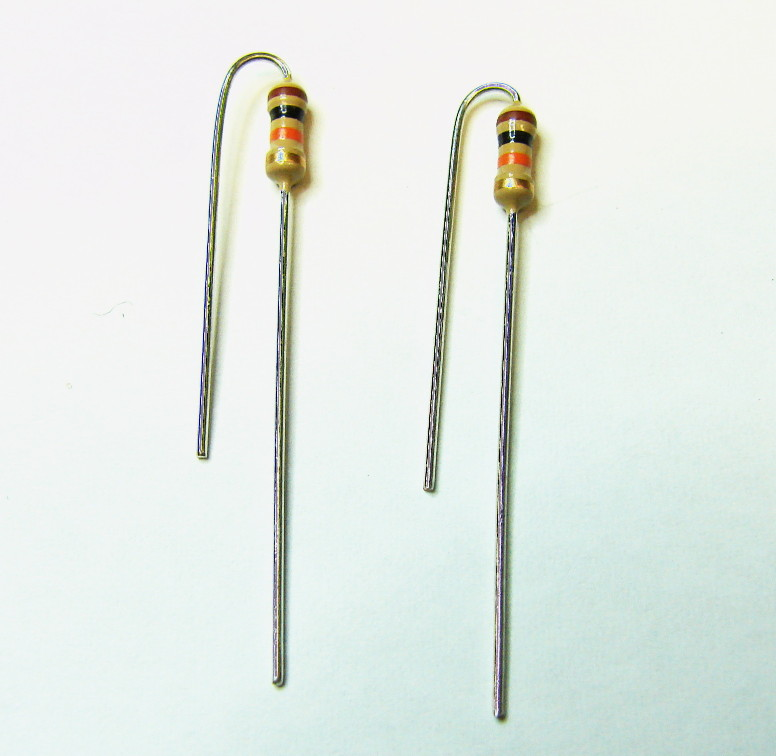
\includegraphics[width=\linewidth]{abb2_1}
\caption{Biegen der Widerstandsdrähte}
\label{fig:abb2_1}
\end{figure}

Anschließend sezen Sie die 150\textOmega-Widerstände entsprechen Abbildung \ref{fig:abb2_2} ein und verlöten Diese. Im nächsten Schritt wiederholen Sie dies mit den 10k\textOmega-Widerständen enstprechend Abbildung \ref{fig:abb2_3}.

\begin{figure}[tbhp]\centering
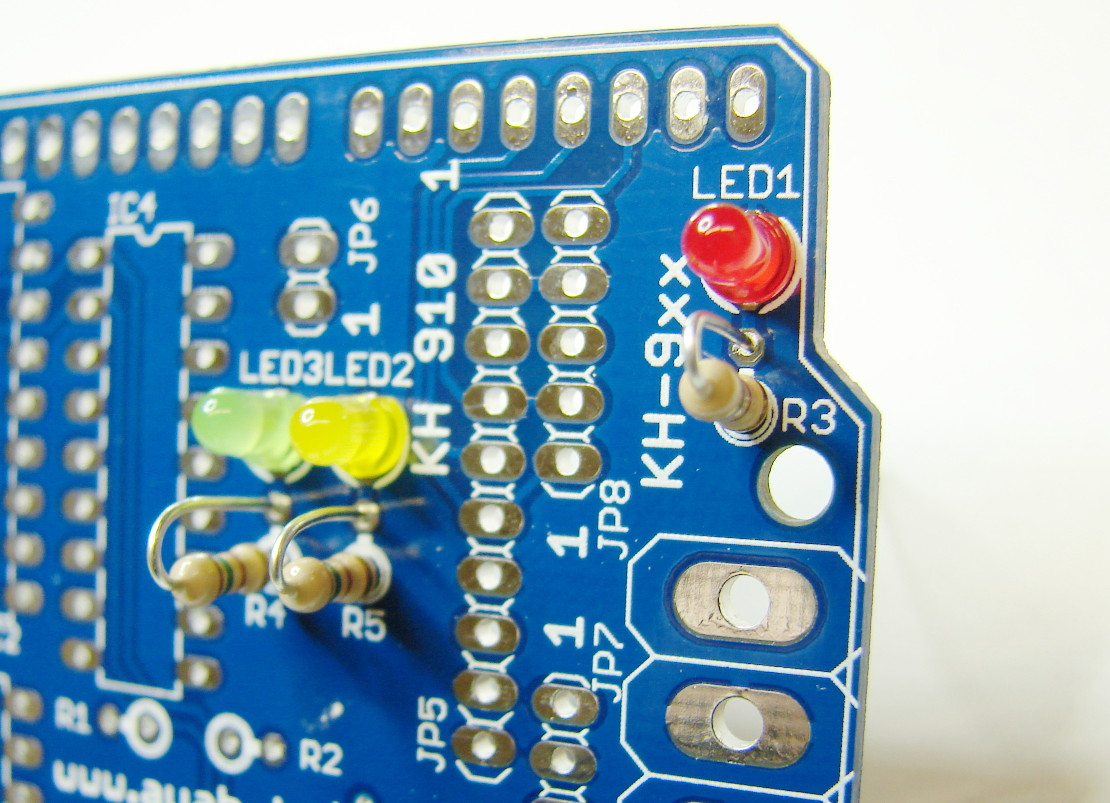
\includegraphics[width=\linewidth]{abb2_2}
\caption{150\textOmega-Widerstände}
\label{fig:abb2_2}
\end{figure}

\begin{figure}[tbhp]\centering
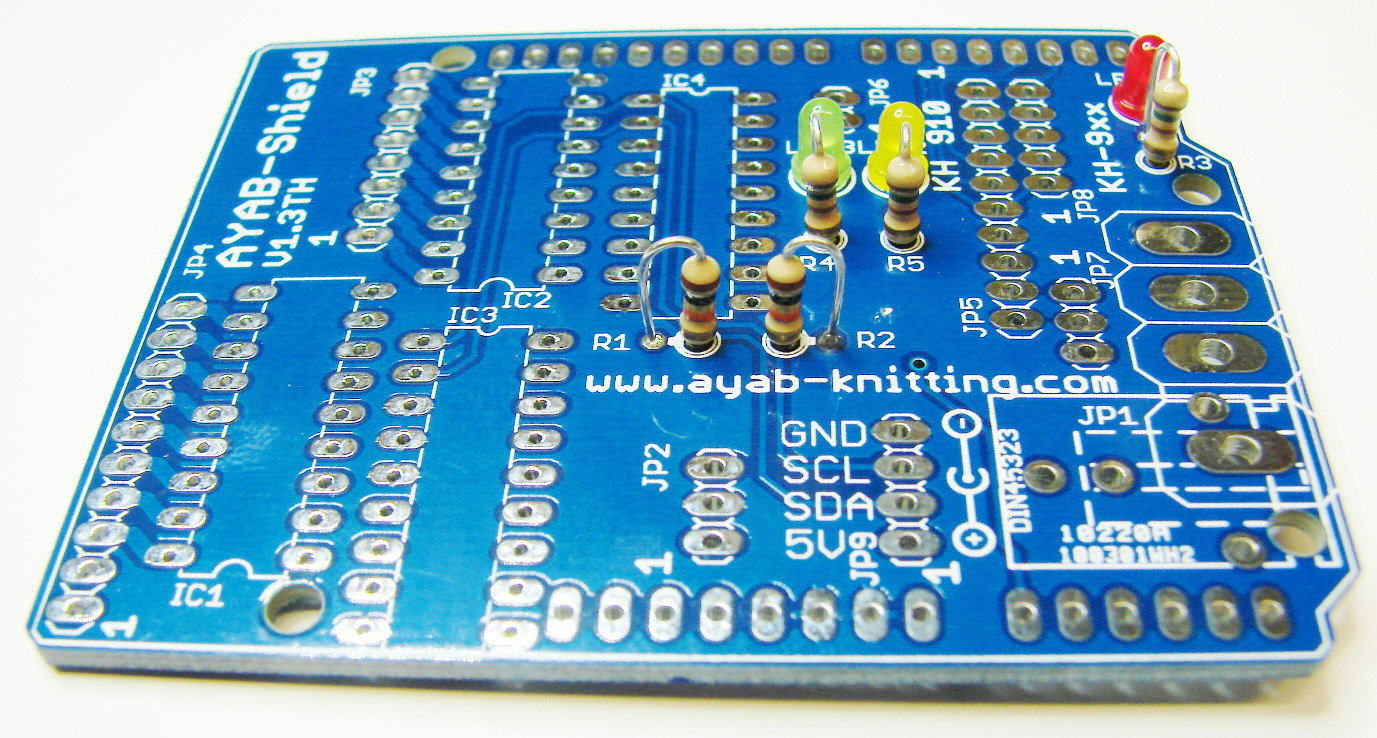
\includegraphics[width=\linewidth]{abb2_3}
\caption{10k\textOmega-Widerstände}
\label{fig:abb2_3}
\end{figure}

\FloatBarrier

 \subsection*{Schritt 3: Maschinenstecker}

\textbf{ACHTUNG!} Dieser Abschnitt wird je nach Maschinentyp unterschiedlich behandelt.\\

\textbf{KH-910 / KH-950:} \\

\begin{tabular}{lll}
\hline
\textbf{Name} & \textbf{Polzahl}  & \textbf{Typ} \\ \hline
JP3           & 8                 & gewinkelt    \\ \hline
JP4           & 10                & gewinkelt    \\ \hline
JP5           & 10                & gerade       \\ \hline
JP9           & 4                 & gerade       \\ \hline
\end{tabular}\\

Verlöten Sie zunächst die Maschinenverbinder JP3, JP4 sowie JP5 entsprechen Abbildung \ref{fig:abb3_1}. Achten Sie dabei darauf JP4 mit etwas Abstand zur Platine zu verlöten (Abbildung \ref{fig:abb3_2}) um das Verbinden mit der Strickmaschine zu erreichtern. Sie konnen dies durch unterlegen eines geeigneten Abstandshalters (z.B. Beilagscheibe) während des Lötvorgangs erleichtern.

\begin{figure}[tbhp]\centering
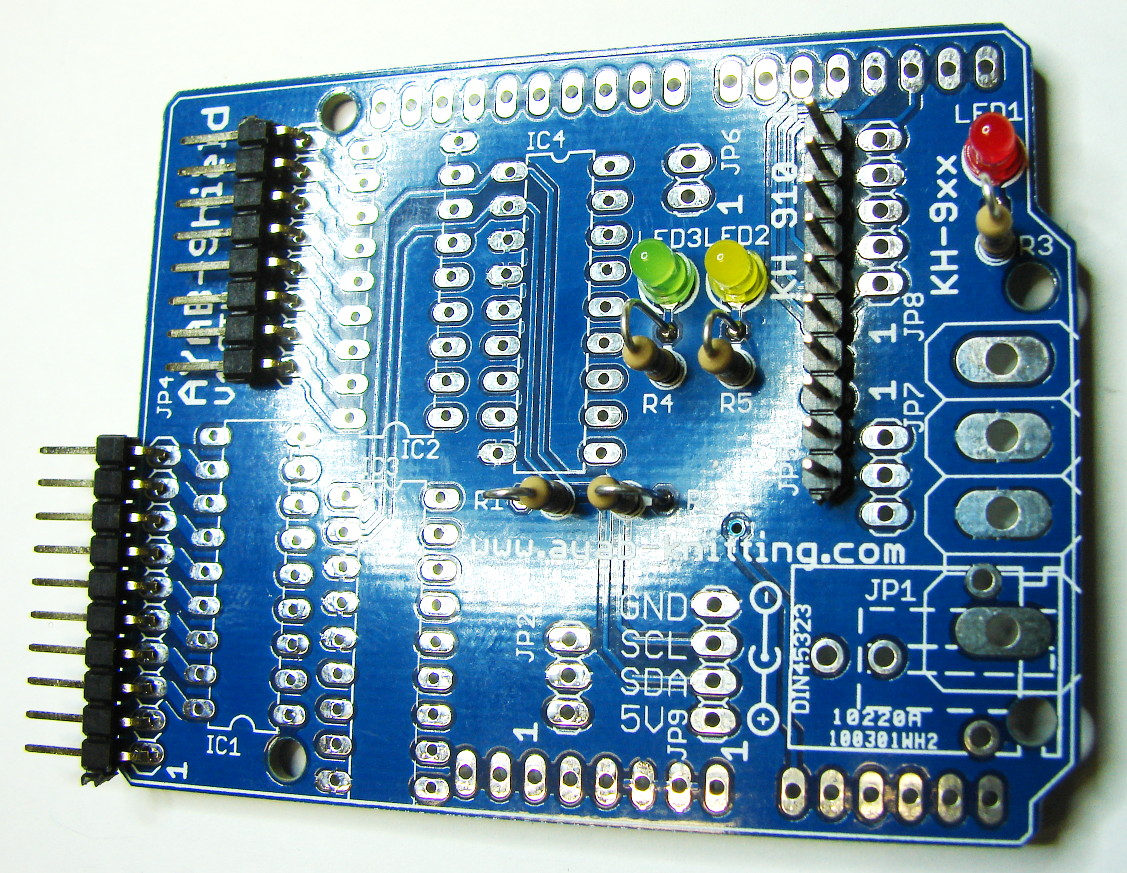
\includegraphics[width=\linewidth]{abb3_1}
\caption{Maschinenverbinder KH-910/KH-950}
\label{fig:abb3_1}
\end{figure}

\begin{figure}[tbhp]\centering
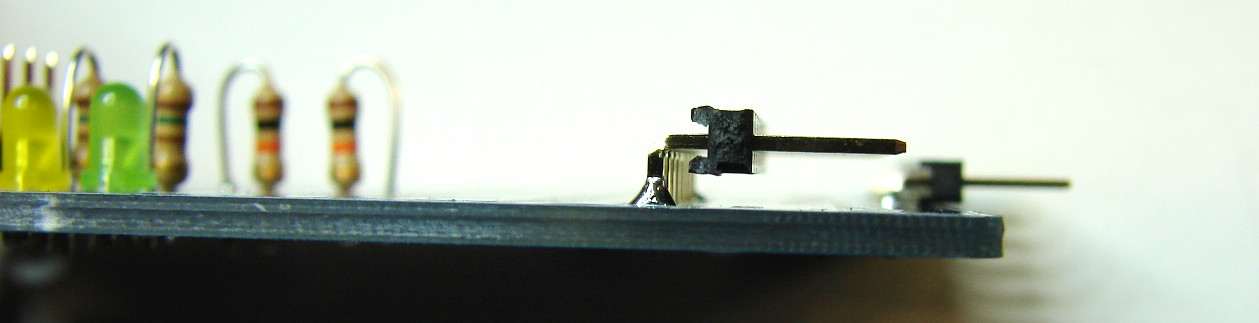
\includegraphics[width=\linewidth]{abb3_2}
\caption{Abstand JP3}
\label{fig:abb3_2}
\end{figure}

Das Anbringen des Erweiterungssteckers JP9 (Abbildung \ref{fig:abb3_3}) kann optional vorgenommen werden. Über diesen Anschluss kann die Funktonalität später durch z.B. eine optionale Farbwechslersteuerung o.ä. ergänzt werden. \par

\begin{figure}[tbhp]\centering
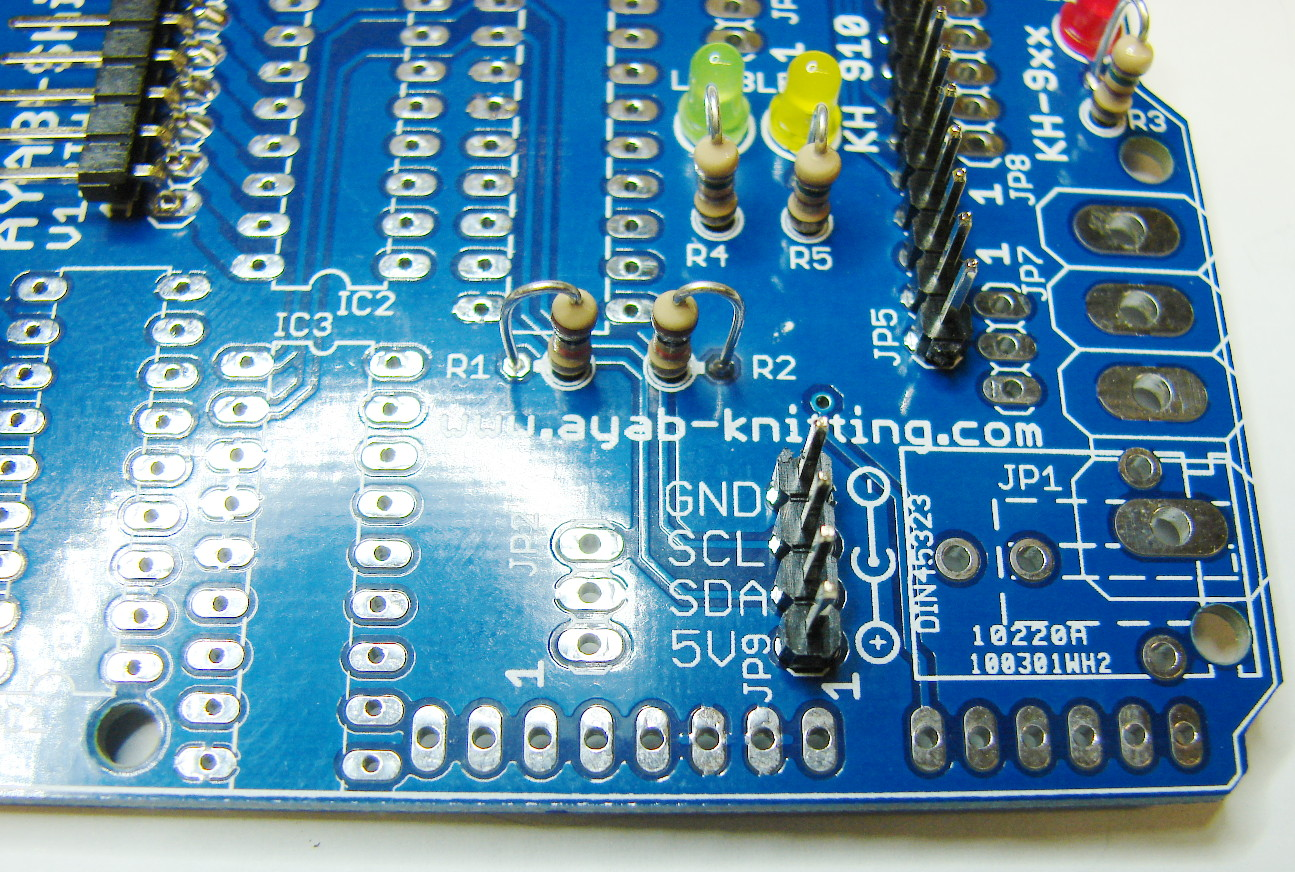
\includegraphics[width=\linewidth]{abb3_3}
\caption{Erweiterungsstecker}
\label{fig:abb3_3}
\end{figure}

\FloatBarrier

\textbf{KH-930:} \\

\begin{tabular}{lll}
\hline
\textbf{Name} & \textbf{Polzahl}  & \textbf{Typ} \\ \hline
JP3           & 8                 & Molex 2.5mm  \\ \hline
JP4           & 10                & Molex 2.5mm  \\ \hline
JP2           & 3                 & Molex 2.5mm  \\ \hline
JP8           & 5                 & Molex 2.5mm  \\ \hline
JP9           & 4                 & gerade       \\ \hline
\end{tabular}\\

Verlöten Sie die Maschinenverbinder JP3, JP4 sowie JP2 und JP8 enstprechend Abbildung \ref{fig:abb3_4}. Achten Sie dabei unbedingt auf die richtige Orientierung der Buchsen (zu erkennen an den dreieckigen Einbuchtungen). Die Einbuchtungen müssen von der roten LED wegzeigen. Achten Sie beim verlöten darauf, dass die Stecker plan auf der Platine aufliegen. Eine nachträgliche Korrektur bei mehrpoligen Steckern gestaltet sich schwierig.

\begin{figure}[tbhp]\centering

\includegraphics[width=\linewidth]{no}
\caption{Maschinenverbinder KH-930}
\label{fig:abb3_4}
\end{figure}

Das Anbringen des Erweiterungssteckers JP9 (Abbildung \ref{fig:abb3_3}) kann optional vorgenommen werden. Über diesen Anschluss kann die Funktonalität später durch z.B. eine optionale Farbwechslersteuerung o.ä. ergänzt werden. \par

\FloatBarrier

 \subsection*{Schritt 4: Piepserstecker}

Nun kann der Stecker für den Piepser wie auf Abbildung \ref{fig:abb4_1} verlötet werden. Auch hier unbedingt auf die Polarität sowie ein planes aufliegen achten.

\begin{figure}[tbhp]\centering
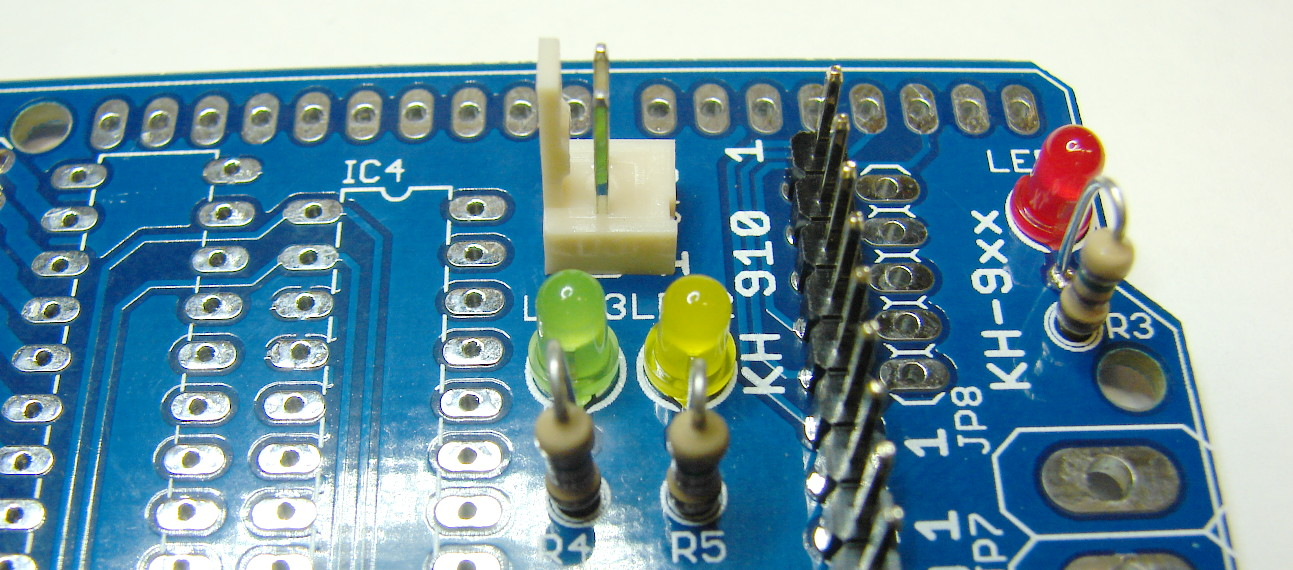
\includegraphics[width=\linewidth]{abb4_1}
\caption{Piepserstecker}
\label{fig:abb4_1}
\end{figure}

\FloatBarrier

 \subsection*{Schritt 5: Arduino Verbindungsstecker}

\textbf{Arduino nicht im Lieferumfang enthalten}\\

Hierfür benötigen Sie folgende Steckverbinder:\\

\begin{tabular}{lll}
\hline
\textbf{Name} & \textbf{Polzahl}  & \textbf{Typ} \\ \hline
ARD1          & 10                & gerade       \\ \hline
ARD2          & 8                 & gerade       \\ \hline
ARD3          & 8                 & gerade       \\ \hline
ARD4          & 6                 & gerade       \\ \hline
\end{tabular}\\


\textbf{Tipp!} Stecken Sie die vier Verbindungsstecker vor dem Verlöten in die Buchsen des Arduinos (Abbildung \ref{fig:abb5_1}) und legen Sie anschließend das AYAB-Shield zum verlöten darauf (Abbildung \ref{fig:abb5_2}). Dies erleichtert die Lötarbeit erheblich und garantiert einen sauberen Verbau. Achten Sie jedoch auf eine möglichst kurze Lötdauer um den Arduino nicht zu beschädigen.

\begin{figure}[tbhp]\centering
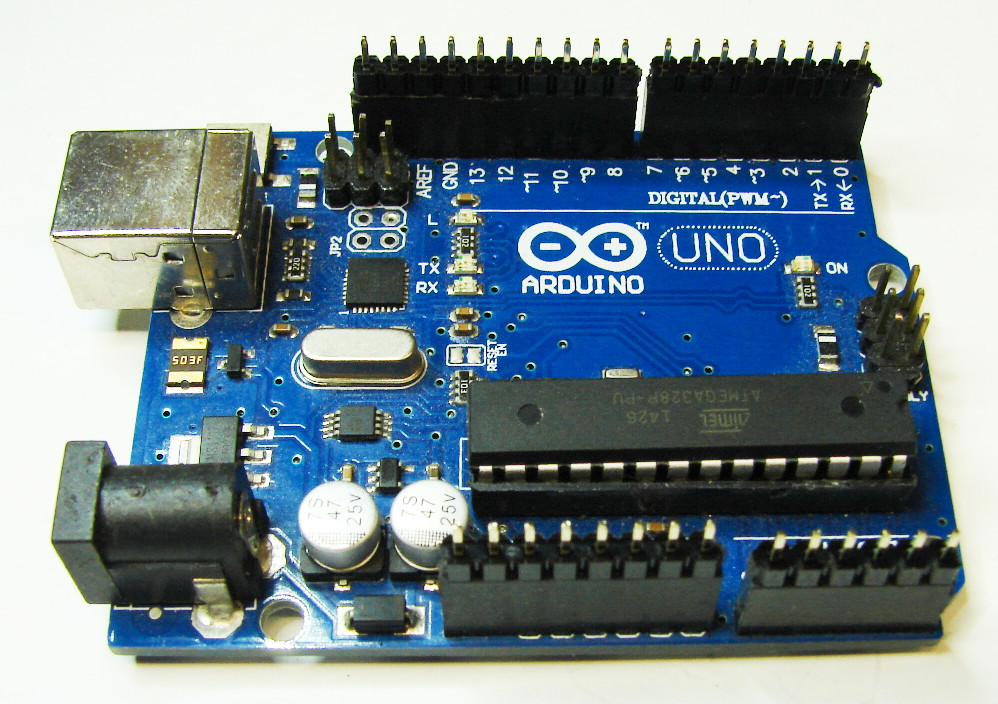
\includegraphics[width=\linewidth]{abb5_1}
\caption{Löterleichterung}
\label{fig:abb5_1}
\end{figure}

\begin{figure}[tbhp]\centering
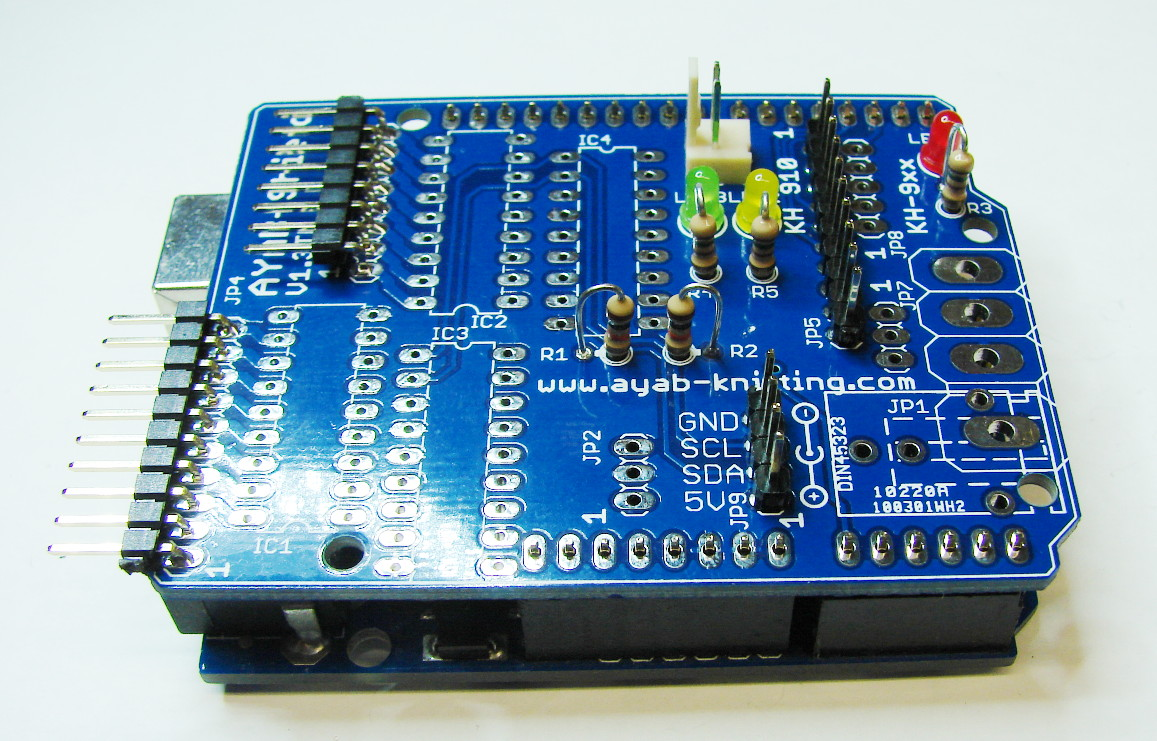
\includegraphics[width=\linewidth]{abb5_2}
\caption{Arduino Verbindungsstecker}
\label{fig:abb5_2}
\end{figure}

\FloatBarrier

 \subsection*{Schritt 6: ICs}

\textbf{Achtung!} Hier unbedingt auf die richtige Orientierung Achten. Die Markierungskerben müssen entsprechend Abbildung \ref{fig:abb6_1} gerichtet sein. Beachten Sie, dass IC1 und IC2 eine andere Orientierung aufweisen als IC3 und IC4. Seien Sie beim einsetzen der ICs behutsam und geduldig. Evtl. müssen die Beinchen sehr vorsichtig etwas nachgebogen werden. Bei zu viel druck können diese leicht brechen. Achten Sie auf eine möglichst kurze Lötdauer um die Bauteile nicht zu überhitzen.\\
\begin{tabular}{ll}
\hline
\textbf{Name} & \textbf{Typ} \\ \hline
IC1           & ULN 2803 L   \\ \hline
IC2           & ULN 2803 L   \\ \hline
IC3           & MCP 23008    \\ \hline
IC4           & MCP 23008    \\ \hline
\end{tabular}\\

\begin{figure}[tbhp]\centering
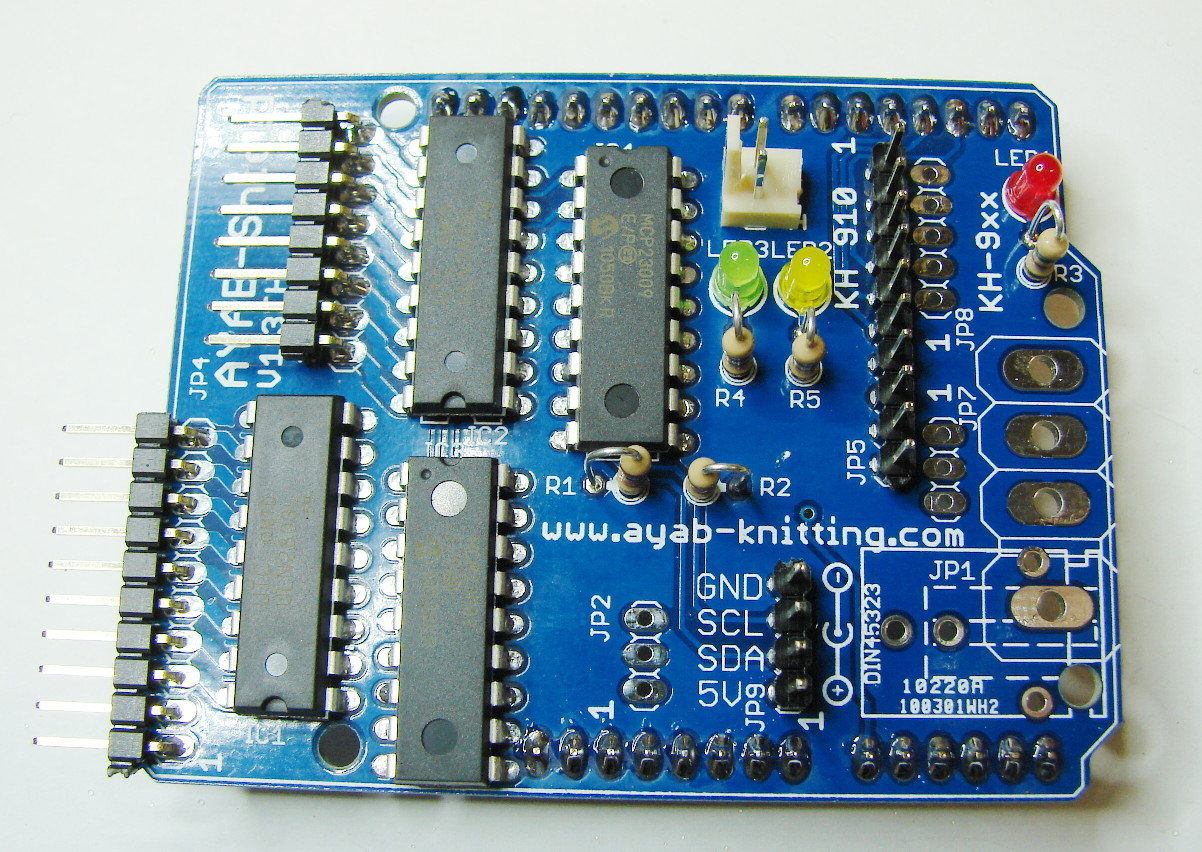
\includegraphics[width=\linewidth]{abb6_1}
\caption{ICs}
\label{fig:abb6_1}
\end{figure}

\FloatBarrier

 \subsection*{Schritt 7: Sensorkabel}

\textbf{ACHTUNG!} Dieser Abschnitt wird je nach Maschinentyp unterschiedlich behandelt.\\

\textbf{KH-910 / KH-950:} \\

Isolieren Sie das Mitgelieferte 3-Adrige Flachbandkabel an beiden Enden entsprechend Abbildung \ref{fig:abb7_1} ab.

\begin{figure}[tbhp]\centering
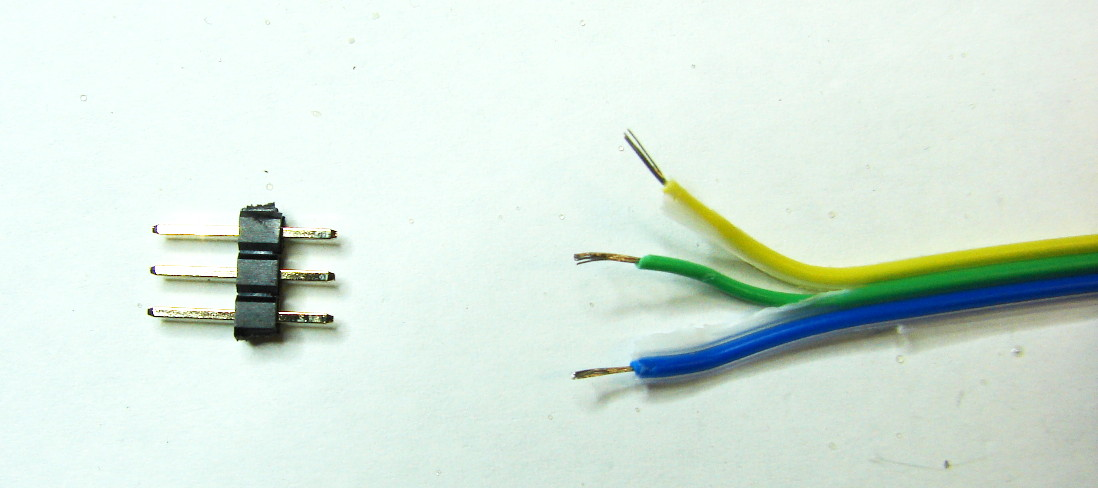
\includegraphics[width=\linewidth]{abb7_1}
\caption{Abisolierung der Kabelenden bei KH-910/KH-950}
\label{fig:abb7_1}
\end{figure}

Verzinnen Sie nun ein Kabelende sowie den 3-poligen Pfostenstecker (Abbildung \ref{fig:abb7_2}) und Verlöten diese anschließend (Abbildung \ref{fig:abb7_3}). Achten Sie hier auf eine gute mechanische Stabilität und prüfen Sie auf evtl. Kurzschlüsse. Sie können zur Verbesserung der Stabilität die offenen Lötstellen einzeln mit Isolierband umwickeln, oder mit einem Schrumpfschlauch fixieren.

\begin{figure}[tbhp]\centering
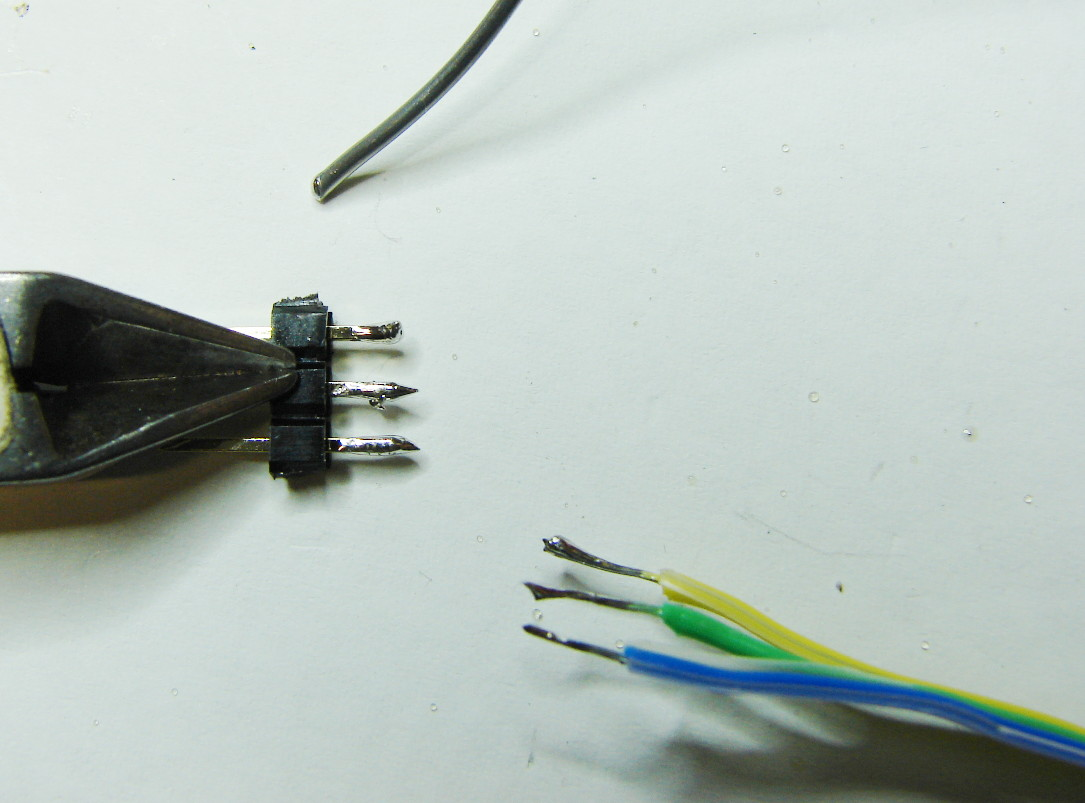
\includegraphics[width=\linewidth]{abb7_2}
\caption{Verzinnung bei KH-910/KH-950}
\label{fig:abb7_2}
\end{figure}

\begin{figure}[tbhp]\centering
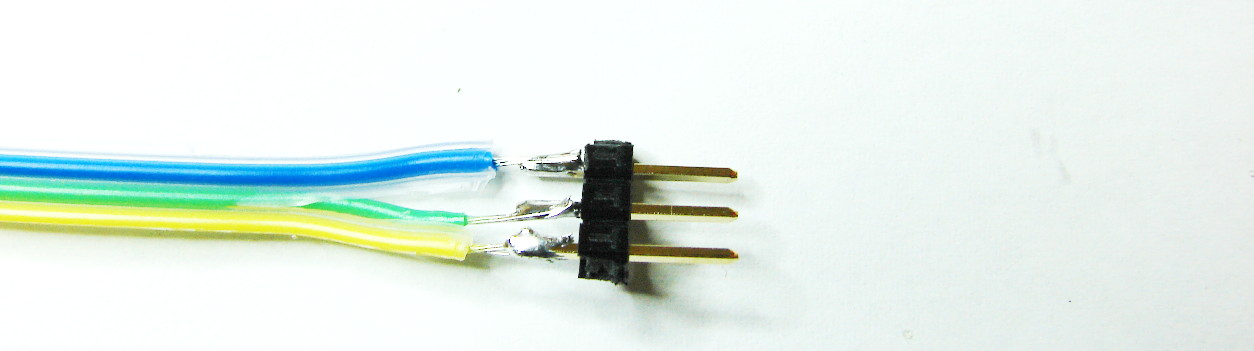
\includegraphics[width=\linewidth]{abb7_3}
\caption{Verlötetes Kabelende bei KH-910/KH-950}
\label{fig:abb7_3}
\end{figure}

Nun verlöten Sie das andere Ende wie auf Abbildung \ref{fig:abb7_4} mit der Platine an JP2 und markieren die Oberseite des Steckers entsprechend. Dies dient zur erleichterung der Orientierung beim Einbau in die Strickmaschine\par

\begin{figure}[tbhp]\centering

\includegraphics[width=\linewidth]{no}
\caption{Verbindung mit Platine bei KH-910/KH-950}
\label{fig:abb7_4}
\end{figure}

\FloatBarrier

\textbf{KH-930:} \\

Isolieren Sie das Mitgelieferte 3-Adrige Flachbandkabel an beiden Enden entsprechend Abbildung \ref{fig:abb7_5} ab.

\begin{figure}[tbhp]\centering

\includegraphics[width=\linewidth]{no}
\caption{Abisolierung der Kabelenden bei KH-930}
\label{fig:abb7_5}
\end{figure}

Verzinnen Sie nun ein Kabelende sowie den 3-poligen Molex-Stecker (Abbildung \ref{fig:abb7_6}) und Verlöten diese anschließend (Abbildung \ref{fig:abb7_7}). Achten Sie hier auf eine gute mechanische Stabilität und prüfen Sie auf evtl. Kurzschlüsse. Sie können zur Verbesserung der Stabilität die offenen Lötstellen einzeln mit Isolierband umwickeln, oder mit einem Schrumpfschlauch fixieren.

\begin{figure}[tbhp]\centering

\includegraphics[width=\linewidth]{no}
\caption{Verzinnung bei KH-930}
\label{fig:abb7_6}
\end{figure}

\begin{figure}[tbhp]\centering

\includegraphics[width=\linewidth]{no}
\caption{Verlötetes Kabelende bei KH-930}
\label{fig:abb7_7}
\end{figure}

Nun verlöten Sie das andere Ende wie auf Abbildung \ref{fig:abb7_8} mit der Platine an JP7. Achten Sie dabei unbedingt auf die richtige Polarität. Das Kabel muss so eingelötet werden, dass von oben der Molex Stecker mit den dreieckigen Einbuchtungen zur roten LED \textbf{hin} zeigt (im Gegensatz zu den anderen Maschinenverbindern).

\begin{figure}[tbhp]\centering

\includegraphics[width=\linewidth]{no}
\caption{Verbindung mit Platine bei KH-930}
\label{fig:abb7_8}
\end{figure}

\FloatBarrier

 \subsection*{Schritt 8: Spannungsversorgung}

\textbf{ACHTUNG!} Dieser Abschnitt wird je nach Maschinentyp unterschiedlich behandelt.\\

\textbf{KH-910 / KH-930 / KH-950 / CK-35:} \\

Bringen Sie den 4-poligen Verbindungstecker entsprechend Abbildung \ref{fig:abb8_1} an und verlöten diesen anschließend. Achten Sie auf eine gleiche höhe der einzelnen Pins und gleichen Sie diese gegebenenfalls vorsichtig aus. Achten Sie darauf, dass die Bodenplatte des Steckers nicht bricht. Durch die dicke der einzelnen Pins, kann es hier etwas länger dauern, bis das Lötzinn sauber verlaufen ist. Verwenden Sie zum halten des Steckers unbedingt eine Zange (Verbrennungsgefahr!).

\begin{figure}[tbhp]\centering

\includegraphics[width=\linewidth]{no}
\caption{Versorgungsstecker KH-910/930/950 und CK35}
\label{fig:abb8_1}
\end{figure}

Im Anschluss müssen die Beinchen an der Unterseite möglichst nahe an der Platine gekürzt werden (Abbildung \ref{fig:abb8_2}) um einen Kurzschluss mit den ISP-Pins des Arduino zu vermeiden.\par

\begin{figure}[tbhp]\centering

\includegraphics[width=\linewidth]{no}
\caption{Kurzschlussvermeidung}
\label{fig:abb8_2}
\end{figure}

\FloatBarrier

\textbf{KH-900 / KH-965:} \\

Verlöten Sie den Hohlstecker entsprechen Abbildung \ref{fig:abb8_3}. \textbf{ACHTUNG!} Die verwendete Polarität trägt den Pluspol an der Außenseite und den Minuspol im Innenleiter. Dies ist die Polarität der original Brother-Netzteile. Bei verwendung von anderen Netzteilen unbedingt auf die richtige Polung achten. Ansonsten kann dies zu Zerstörung von Bauteilen oder gar der Strickmaschine führen.

\begin{figure}[tbhp]\centering

\includegraphics[width=\linewidth]{no}
\caption{Versorgungsstecker KH-900/965}
\label{fig:abb8_3}
\end{figure}

\FloatBarrier

 \subsection*{Abschließende Kontrolle}

Kontrollieren Sie nochmal vor Inbetriebnahme der Schaltung, ob alle Bauteile richtig eingesetzt und gepolt sind. Sehen Sie auf der Lötseite (Leiterbahnseite) nach, ob durch Lötzinnreste Leiterbahnen überbrückt wurden, da dies zu Kurzschlüssen und zur Zerstörung von Bauteilen führen kann. Ferner ist zu kontrollieren, ob abgeschnittene Drahtenden auf oder unter der Platine liegen, da dies ebenfalls zu Kurzschlüssen führen kann.
Kontrollieren sie alle Lötstellen auf sauberkeit der Ausführung. Kalte Lötstellen oder Lötbrücken beeinträchtigen die Funktion und können zu Zerstörung von Bauteilen oder gar der Strickmaschine führen.

%------------------------------------------------

\section{Funktionstest und Inbetriebnahme}

 \subsection*{Checkliste}

\begin{itemize}[noitemsep] % [noitemsep] removes whitespace between the items for a compact look
\item[\Square] offener Punkt
\item[\XBox] angekreuzter Punkt
\item[\CheckedBox] abgehakter Punkt
\end{itemize}

 \subsection*{Verhalten bei Störungen}

%------------------------------------------------

\section{Gewährleistung}

Da wir keinen Einfluss auf den richtigen und sachgemäßen Aufbau haben, können wir aus verständlichen Gründen bei Bausätzen nur die Gewähr der Vollständigkeit und einwandfreien Beschaffenheit der Bauteile übernehmen.

Garantiert wird eine den Kennwerten entsprechende Funktion der Bauelemente im uneingebautem Zustand und die Einhaltung der technischen Daten der Schaltung bei entsprechend der Lötvorschrift,
fachgerechter Verarbeitung und vorgeschriebener Inbetriebnahme und Betriebsweise.

Weitergehende Ansprüche sind ausgeschlossen.

Wir übernehmen weder eine Gewähr noch irgendwelche Haftung für Schäden oder Folgeschäden im Zusammenhang mit diesem Produkt.

Wir behalten uns eine Reparatur, Nachbesserung, Ersatzteillieferung oder Rückerstattung des Kaufpreises vor.

Bei folgenden Kriterien erfolgt keine Reparatur bzw. es erlischt der Gewährleistungsanspruch:

\begin{itemize}[noitemsep] % [noitemsep] removes whitespace between the items for a compact look
\item wenn zum Löten säurehaltiges Lötzinn, Lötfett oder säurehaltiges Flussmittel u. ä. verwendet wurde.
\item wenn der Bausatz unsachgemäß gelötet und aufgebaut wurde.
\item bei Veränderung und Reparaturversuchen am Gerät
\item bei eigenmächtiger Abänderung der Schaltung
\item bei der Konstruktion nicht vorgesehene, unsachgemäße Auslagerung von Bauteilen, Freiverdrahtung von Bauteilen wie Schalter, Potis,
Buchsen usw.
\item Verwendung anderer, nicht original zum Bausatz gehörender Bauteile
\item bei Zerstörung von Leiterbahnen oder Lötaugen
\item bei falscher Bestückung und den sich daraus ergebenden Folgeschäden
\item bei Überlastung der Baugruppe
\item bei Schäden durch Eingriffe fremder Personen
\item bei Schäden durch Nichtbeachtung der Bedienungsanleitung und des Anschlussplanes
\item bei Anschluss an eine falsche Spannung oder Stromart
\item bei Falschpolung der Baugruppe
\item bei Fehlbedienung oder Schäden durch fahrlässige Behandlung oder Mißbrauch
\item bei Defekten, die durch überbrückte Sicherungen oder durch Einsatz falscher Sicherungen entstehen
\end{itemize}

In all diesen Fällen erfolgt die Rücksendung des Bausatzes zu Ihren Lasten.

Beim Umgang mit Produkten, die mit elektrischer Spannung in Berührung kommen, müssen die güitigen VDE-Vorschriften beachtet werden, insbesondere VDE 0100, VDE055010551, VDE 0700, VDE 0711
und VDE 0860.

%------------------------------------------------

\section{Anhang}

 \subsection*{Bauteile und Bestellnummern}

 \subsection*{Schaltplan}

 \subsection*{Bestückungsplan}

%------------------------------------------------

\phantomsection
\section*{Impressum} % The \section*{} command stops section numbering

\addcontentsline{toc}{section}{Impressum} % Adds this section to the table of contents

\begin{figure}[tbhp]

\includegraphics[width=0.3\linewidth]{cc}
\end{figure}

\textbf{Anschrift:}

thinkstack UG

Türkenstraße 21

80799 München

https://thinkstack.de



%----------------------------------------------------------------------------------------
%	REFERENCE LIST
%----------------------------------------------------------------------------------------
\phantomsection
\bibliographystyle{unsrt}
%\bibliography{sample}

%----------------------------------------------------------------------------------------

\end{document}
